\documentclass[11pt,a4paper]{article}
\usepackage[utf8]{inputenc}
\usepackage[czech]{babel}
\usepackage[T1]{fontenc}
\usepackage{amsmath}
\usepackage{amsfonts}
\usepackage{listings}
\usepackage{color}
\usepackage{epstopdf}
\usepackage{svg}
\usepackage{url}
\usepackage{amssymb}
\usepackage{graphicx}
\bibliographystyle{documentation}
\usepackage[left=2cm,right=2cm,top=2.5cm,bottom=2cm]{geometry}
\author{Tomáš Kohout, Tomáš Blažek}
\begin{document}


\DeclareGraphicsExtensions{.pdf,.png,.jpg}

\newcommand{\slideRef}[1]{\textit{(IMS slide #1)}}
\newcommand{\code}[1]{\texttt{#1}}

	\begin{titlepage}

		\begin{center}

			\textsc{
				\Huge
					Vysoké učení technické v~Brně\\
				\huge
					Fakulta informačních technologií
			}\\

			\vspace{\stretch{0.320}}

			\LARGE
					IMS - Modelování a simulace\\
					4. Doprava zboží nebo osob\\~\\
			\Huge{}
					Dokumentace
			\vspace{\stretch{0.650}}

		\end{center}

		{\Large
			29. listopadu 2017
			\hfill
			Tomáš Blažek, Tomáš Kohout
		}

	\end{titlepage}

	\tableofcontents

	\pagebreak


	\section{Úvod a motivaci}
	Tato práce si klade za cíl zjistit, zda dosavadní frekvence převážení cestujících přívozem na trase Podbaba-Podhoří je v
  souladu s množstvím přepravovaných osob nebo zda je možné tuto frekvenci snížit. Na základě vytvořeného modelu
  budou provedeny experimenty s různými časovými úseky a různým množstvím cestujících.

  Tato práce si klade za cíl zjistit, zda je dosavadní frekvence převážení cestujících přívozem na trase Podbaba-Podhoří
  v souladu s množstvím převážených cestujících. Pro tento účel byl vytvořen model (\cite{SLAJD}, 7. slide)

	\subsection{Konzultace a zdroje}
	Autory projektu jsou Tomáš Blažek a Tomáš Kohout. Pro vytvoření projektu jsou použity veřejně dostupné informace ze stránek Dopravního podnku hl. m. Prahy, především pak jízdní řád a informace o celkovém počtu přepravených osob. Abstraktní model je vytvořen na základě jizdního řádu a pozorování .

	\subsection{Ověřování validity modelu}
  Model byl ověřován experimenty prováděné pomocí modelu. Získané výsledky byly následně porovná-
  vány s reálnými údaji získanými na základě pozorování obsluhy pasažérů \cite{DELKA_CESTY} a také pomocí získaných dat \cite{ROCENKY}. 

	\section{Rozbor tématu a použitých metod/technologií}
  Pro modelování a následnou simulaci přívozu je nezbytné znát jeho reálné chování.
  Přívoz z Podbaby do Podhoří se zabývá výlučně přepravou cestujících z jednoho
  břehu na druhý. Tuto informaci jsme získali pozorováním z následujícího videa \cite{DELKA_CESTY}.
  Z toho samého snímku je patrná i doba cesty, která je v tomto konkrétním případě 1 minuta a 28 sekundy
  Na stejném videu jsme také vypozorovali průměrnou dobu vystupování. Ta se pohybuje
  okolo 5 sekund v případě staršího typu lodě, který je vidět na videu. V současné době je ovšem používána loď zakoupená
  v roce 2016 \cite{LOD}, která má palubu v rovině s molem a vyšší kapacitu. Kapacita se z původních 12 míst zvýšila na
  40. Dále bylo nutné zjistit celkový počet jízd přívozu za jeden pracovní den. Tuto informaci
  jsme zjistili z jízdního řádu \cite{PID}, který je platný od 11.12.2016.
  V ročenkách Technické správy komunikací hl. m. Prahy jsme získali data potřebná pro
  správné generování cestujících \cite{ROCENKY}. Tato hodnota se pohybuje v rozsahu od 190 000
  až po 350 000 převezených cestujících ročně. Předpokládáme, že v letním období je
  zájem o přepravu přívozem větší než v zimě. Nejsou však k dispozici žádné informace o
  počtu převezených pasažérů v letním období, budeme tedy uvažovat, že v letním období
  převeze přívoz denně přibližně 2 - 3 krát více osob než v zimnímm období.

  \subsection{Použíté postupy pro vytváření modelu}
  Postup se skládá z několika kroků. Nejprve bylo nutné dekomponovat úlohu na jednotlivé procesy,
  které se v ní odehrávají. Petriho síť(\cite{SLAJD}, slide 123-142), byla vhodným kandidátem pro grafické znázornění
  jednotlých procesů, ze které se dále vycházelo při tvorbě simulačního modelu.

  \subsection{Původu použitých metod/technologií}
  Pro vytvoření simulačního modelu byl použitý jazyk C++, neboť v tomto jazyce je napsaná knihovna SIMLIB \cite{SIMLIB},
  která je vhodná pro vytvoření simulačního modelu daného problému, protože obsahuje funkce, které vystihují
  chování systému hromadné obsluhy. V modelu jsou použity algoritmy využívané v příkladech na democvičení \cite{DEMOCVIKO}.

  \section{Koncepce modelu}
  Smyslem tohoto projektu je simulovat (\cite{SLAJD}, slide 8) provoz přívozu Pražské integrované dopravy
  z Podbaby do Podhoří v určitém časovém intervalu a sledovat zahlcenost nebo nezahlcenost kapacity přívozu,
  popřípadě délku front na obou březích a vytvořit tak ideální frekvenci jízd.

  Zanedbali jsme povodňové stavy a různé poruchy, protože pro simulaci (\cite{SLAJD}, slide 8)
  jsou marginální. Přívoz při prvním povodňovém stupni nevyjíždí a poruchy různého druhu se
  můžou vyskytnout, ale pro zjištění frekvence jízd nejsou podstatné.

  \subsection{Návrh konceptuálního modelu}
  Přívoz má dvě mola. Ke každému molu přicházejí cestující s exponenciálním rozložením (\cite{SLAJD}, slide 91).
  Tito cestující čekají na uvolnění mola. Je-li molo k dispozici, není vyčerpána kapacita lodě a nenastal čas odjezdu
  nastupují po jednom pasažérovi do lodě. Nastupování samo o sobě zabere určitý čas. Pokud nastane čas odjezdu, tak právě
  nastupující cestující dokončí svou činnost a loď vypluje na cestu. Po určité době dojede k druhému molu, kde nejprve vystoupí naložení cestující.
  Následně mohou nastupovat čekající cestující. Nastupování probíhá totožně jako na prvním molu.
  Po uplynutí určité doby a dokončeném nastupování pasažéra, který nastupoval v době odjezdu odjede loď zpět k
  prvnímu molu, kde opět vyloží naložené cestující a celý proces se opakuje. Doba čekání na druhém břehu musí být
  dostatečná pro vystoupení a nastoupení plně obsazené lodě.

  \subsection{Forma konceptuálního modelu}

  Pro popis abstraktního modelu (\cite{SLAJD}, slide 40-43) byla vytvořena Petriho síť (\cite{SLAJD}, slide 123-142),
  ze získaných informací uvedených dříve v textu. Tato síť je hierarchicky popsána na obrázcích \ref{pnTime}, \ref{pnWork} a \ref{pnWork2}.

	\begin{figure}[h]
		\centering
		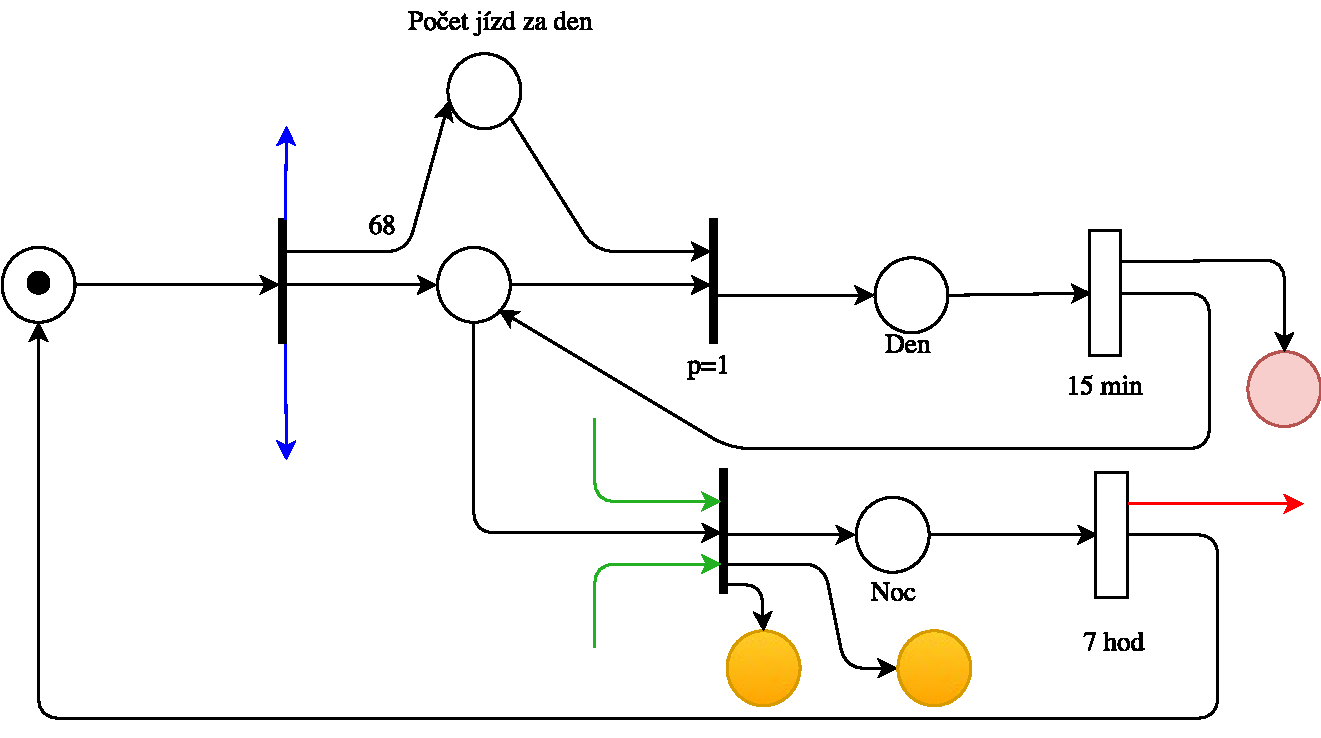
\includegraphics[scale=0.7]{pn-daytime.pdf}
		\caption{Petriho síť znázorňující režim odjezdů}
		\label{pnTime}
	\end{figure}

	Na obrázku \ref{pnTime} vidíme, že v původním jízdní řádu je počet jízd udán číslem 68 a
	poté následuje 7 hodin pauza. Modré šipky indikují začátek generování nových pasažérů.
	Zelené šipky indikují ukončení generování pasažérů přes noc. Do zlata zbarevé stavy
	slouží k vyprázdnění fronty čekajících pasažérů na odvoz, aby nečekali přes noc.
	Červená šipka uvolní molo Podhoří a umožní cestujícím nastupovat. Do červena zbarvený
	stav určuje, že po nastoupení posledního pasažéra se vydají naložení pasažéři na cestu.

	\begin{figure}[h]
		\centering
		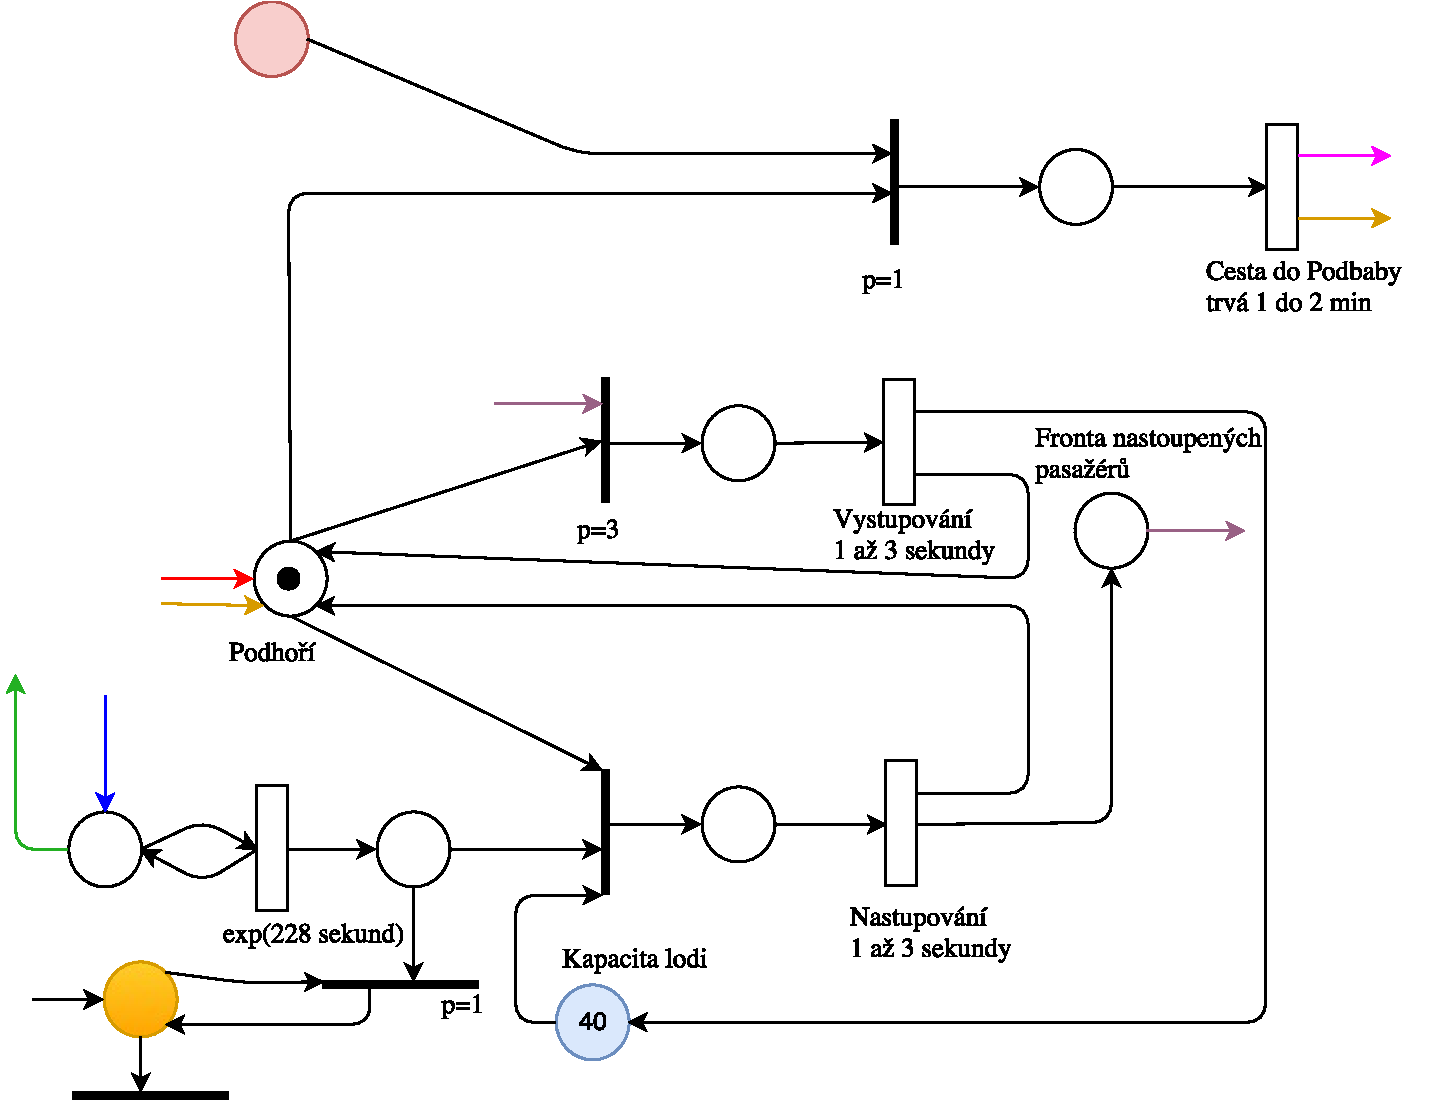
\includegraphics[scale=0.7]{pn-work.pdf}
		\caption{Petriho síť znázorňující nástup/výstup pasažérů a cestu ke druhému molu}
		\label{pnWork}
	\end{figure}

	\newpage
	Na obrázku \ref{pnWork} je znázorněno nastupování a vystupování cestujících. Pokud nastane čas
	odjezdu, tak se loď vydá na cestu a pluje ke druhému molu. Z obrázku je zřejmé, že vždy dojde
	nejprve k vystoupení cestujících a až posléze k nastoupení nových pasažérů, přičemž k odejzdu
	dojde až poté, co nastoupí poslední cestující. Celý abstraktní model používá pouze jednu kapacitu lodě.
	Na obrázku \ref{pnWork} a obrázku \ref{pnWork2} je znázorněn světle modrou barvou.
	Generování cestujících začíná vždy se začátkem nového dne a končí s koncem dne.
	Na konci dne se všichni čekající cestující uvolní ze systému (\cite{SLAJD}, slide 7).

	\begin{figure}[h]
		\centering
		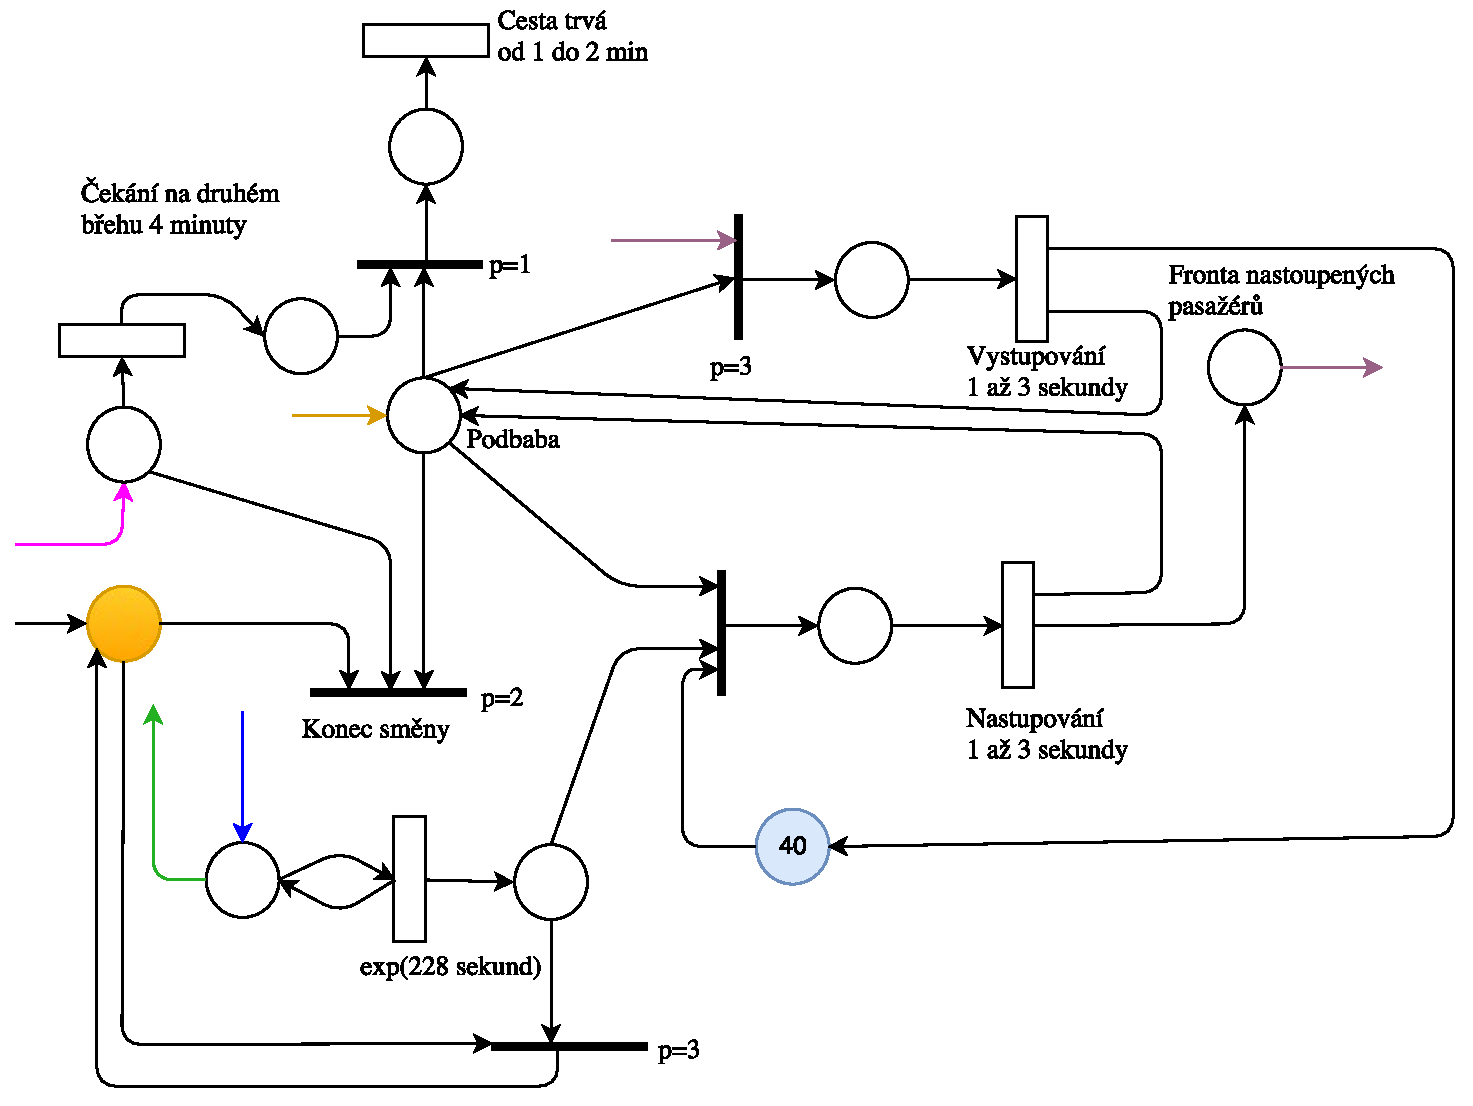
\includegraphics[scale=0.7, width=\textwidth]{pn-work2.pdf}
		\caption{Petriho síť znázorňující nástup/výstup pasažérů a cestu k prvnímu molu}
		\label{pnWork2}
	\end{figure}
	Zde vidíme, že po příjezdu do Podbaby se vytvoří nový proces, který čeká 4 minuty.
	Po uplynutí této doby se loď vydá zpět na cestu do Podhoří. V tomto čase stihne vyložit
	cestujícící a naložit nové. Pokud je tato jízda poslední, tak je proces lodi ze systému (\cite{SLAJD}, slide 7) uvolněn.
	Stejně tak jsou uvolněni i pasažéři, kteří nemohou být naloženi z důvodu noční fáze.

 \newpage
	\section{Architektura simulačního modelu}
	V programu jsou implementovány 2 Facility(\cite{SLAJD}, slide 163). Ty reprezentují 2 mola, které umožňují nástup cestujících.
    Dále jeden prvek typu Store(\cite{SLAJD}, slide 163), který znázoruňuje palubu lodi s určitou kapacitou. V samotném simulačním
	modelu (\cite{SLAJD}, slide 9) jsou využívány 2 generátory pasažérů rozšiřující třídu Event((\cite{SLAJD}, slide 163)). Ty se starají o generování
	pasažérů na obou březích. Jelikož v reálném světě přicházejí cestují pouze přes den v pracovní době přívozu,
	tak je generování pasažérů v hodinách mimo pracovní dobu pozastaveno a na začátku pracovní doby opět spuštěno.
	Pasažéři jsou dvou typů, rozlišují se ve směru jízdy. Ti jsou implementovány jako třídy, které jsou rozšířené
	třídou Process(\cite{SLAJD}, slide 163). Při vygenerování pasažéra, je jeho první činnost zjistit, zda je možné využít molo k nástupu
	do přistavené lodi nebo se postavit do čekací fronty. Celé toto řidí proces času, který znázorňuje
	dopravní řád přívozu a určuje kdy mohou pasažeři nastupovat či vystupovat.

	\section{Podstata simulačních experimentů a jejich průběh}

	Cílem experimentů je najít vhodný jízdní řád pro přívoz na trase Podbaba - Podhoří v Praze.
	Ke zjištění této informace je vhodné vytvořit model (\cite{SLAJD}, slide 7),
	neboť provádění experimentů při ostrém provozu není možné z důvodu platných smluvních
	podmínek Pražského dopravního podniku, které jsou uzavřeny s každým cestujícím, který
	si zakoupí jízdenku.
	\subsection{Postup experimentů}
  V simulačním modelu jsou možné úpravy u následujících hodnot.
	\begin{enumerate}
		\item Určení rychlosti generování pasažérů.
		\item Počet jízd přívozu
		\item Kapacitu lodi
	\end{enumerate}

	Pro vytvoření nejvhodnější frekvence jízd jsme se rozhodli ovlivnit rychlost
	generování pasažérů, počet jízd za den a kapacitu lodi pro převoz pasažérů mimo
	sezónu.

	\subsection{Jednotlivé experimenty}

	\subsubsection{Experiment 1}






	\section{Závěr}

	\newpage
	\section{Zdroje}
		\bibliography{documentation}


\end{document}
